% poster cientifico slumx botnet analysis
\documentclass[25pt, a0paper, portrait]{tikzposter}

% paquetes necesarios
\usepackage[utf8]{inputenc}
\usepackage[english]{babel}
\usepackage{lmodern}
\usepackage{amsmath}
\usepackage{amsfonts}
\usepackage{amssymb}
\usepackage{graphicx}
\usepackage{booktabs}
\usepackage{array}
\usepackage{multirow}
\usepackage{xcolor}
\usepackage{colortbl}
\usepackage{pgfplots}
\pgfplotsset{compat=1.17}
\usetikzlibrary{arrows.meta, positioning, shapes.geometric, fit, calc, shadows, backgrounds}

% ==============================================================================
% DEFINICIÓN DE COLORES (DARK MODE / NEON ACCENTS)
% ==============================================================================
\definecolor{DarkBackground}{HTML}{0B1120} % Deep Navy/Black
\definecolor{BlockBackground}{HTML}{1E293B} % Slate 800
\definecolor{TextWhite}{HTML}{F1F5F9}       % Slate 100
\definecolor{AccentCyan}{HTML}{22D3EE}      % Cyan 400
\definecolor{AccentBlue}{HTML}{60A5FA}      % Blue 400
\definecolor{AccentPurple}{HTML}{C084FC}    % Purple 400
\definecolor{AccentGreen}{HTML}{4ADE80}     % Green 400
\definecolor{AccentRed}{HTML}{F87171}       % Red 400
\definecolor{AccentOrange}{HTML}{FB923C}    % Orange 400

% ==============================================================================
% ESTILO DEL POSTER
% ==============================================================================
\definecolorstyle{DarkNeonStyle}{
    \definecolor{colorOne}{named}{AccentCyan}
    \definecolor{colorTwo}{named}{AccentBlue}
    \definecolor{colorThree}{named}{AccentPurple}
}{
    % Background
    \colorlet{backgroundcolor}{DarkBackground}
    \colorlet{framecolor}{DarkBackground}
    % Title
    \colorlet{titlefgcolor}{TextWhite}
    \colorlet{titlebgcolor}{DarkBackground}
    % Block
    \colorlet{blocktitlebgcolor}{BlockBackground}
    \colorlet{blocktitlefgcolor}{AccentCyan}
    \colorlet{blockbodybgcolor}{BlockBackground}
    \colorlet{blockbodyfgcolor}{TextWhite}
    % Inner Block
    \colorlet{innerblocktitlebgcolor}{AccentBlue!20}
    \colorlet{innerblocktitlefgcolor}{TextWhite}
    \colorlet{innerblockbodybgcolor}{DarkBackground}
    \colorlet{innerblockbodyfgcolor}{TextWhite}
    % Note
    \colorlet{notefgcolor}{DarkBackground}
    \colorlet{notebgcolor}{AccentCyan}
    \colorlet{noteframecolor}{AccentCyan}
}

% Custom Title Style
\definetitlestyle{SimpleTitle}{
    width=\paperwidth, roundedcorners=0, linewidth=0pt, innersep=2cm,
    titletotopverticalspace=0mm, titletoblockverticalspace=20mm
}{
    \draw[draw=none, fill=titlebgcolor] (\titleposleft,\titleposbottom) rectangle (\titleposright,\titlepostop);
}

% Custom Block Style (Clean Dark Card with Glow/Shadow)
\defineblockstyle{DarkCard}{
    titlewidthscale=1, bodywidthscale=1, titleleft,
    titleoffsetx=0pt, titleoffsety=0pt, bodyoffsetx=0pt, bodyoffsety=0pt,
    bodyverticalshift=0pt, roundedcorners=10, linewidth=0pt,
    titleinnersep=15pt, bodyinnersep=15pt
}{
    \begin{scope}[drop shadow={fill=black, shadow xshift=3pt, shadow yshift=-3pt, opacity=0.6}]
        \fill[color=blockbodybgcolor, rounded corners=10pt] (blockbody.south west) rectangle (blockbody.north east);
        \ifBlockHasTitle
            % Optional: Add a thin accent line under the title
            \draw[color=AccentCyan, line width=2pt] ([yshift=-2pt]blocktitle.south west) -- ([yshift=-2pt]blocktitle.south east);
        \fi
    \end{scope}
}

\usecolorstyle{DarkNeonStyle}
\usetitlestyle{SimpleTitle}
\useblockstyle{DarkCard}

% ==============================================================================
% TÍTULO
% ==============================================================================
\makeatletter
\settitle{
    \parbox{\linewidth}{
        \centering
        \begin{minipage}{0.12\linewidth}
            \centering
            
\includegraphics[width=\linewidth, height=6cm, keepaspectratio]{university_logo.png}
        \end{minipage}%
        \begin{minipage}{0.74\linewidth}
            \centering
            \color{titlefgcolor}
            {\bfseries \LARGE \@title}\\[1em]
            {\Large \@author}\\[0.5em]
            {\large \@institute}
        \end{minipage}%
        \begin{minipage}{0.12\linewidth}
            \centering
            ~ % Invisible character to maintain symmetry
        \end{minipage}
    }
}
\makeatother

\title{Analysis of IoT Botnet Structure and Behavior: A Study Based on the Hitori (SlumX) Variant}
\author{Ariel Matias Melo Pazmiño}
\institute{Universidad Internacional del Ecuador - Facultad de Ciencias Técnicas}

% ==============================================================================
% DOCUMENTO
% ==============================================================================
\begin{document}

\maketitle

\begin{columns}

    % ==========================================================================
    % COLUMNA 1
    % ==========================================================================
    \column{0.33}

    \block{Abstract}{
        \normalsize
        This research presents a comprehensive technical analysis of the SlumX botnet (Hitori variant), elaborating on its architecture, attack vectors, and operational patterns through static code analysis. The study unmasks a sophisticated Command and Control (C2) mechanism, diverse DDoS attack methods (UDP, TCP, HTTP), and advanced evasion techniques unique to IoT devices [1]. Key findings include the identification of multi-architecture support (MIPS, ARM, x86, etc.) and the evolution of Mirai-driven botnets toward more complex infrastructures with increased persistence [2]. This work contributes to cybersecurity research by documenting modern IoT botnet behaviors and suggesting mitigation strategies [5].
        
        \vspace{0.8em}
        \noindent\colorbox{BlockBackground}{\parbox{0.96\linewidth}{\normalsize\color{AccentCyan}
        \textbf{Key Focus:} Understanding the evolution from simple credential attacks to sophisticated multi-architecture IoT malware with advanced evasion capabilities.
        }}
    }

    \block{Research Objectives}{
        \normalsize
        This study aims to dissect the operational mechanics of the SlumX botnet, a variant of the infamous Mirai malware [1]. By analyzing the source code, we identify the specific modifications that allow it to target a wider range of IoT devices compared to its predecessors.

        \vspace{0.5em}
        \textbf{\large\color{AccentBlue}Specific Objectives}
        \vspace{-0.2em}
        \begin{itemize}\setlength\itemsep{0.3em}
            \item Analyze core architecture and operational framework.
            \item Examine Command \& Control infrastructure design.
            \item Identify and categorize DDoS attack vectors [3].
            \item Evaluate multi-architecture support mechanisms.
            \item Document evasion and anti-analysis techniques.
        \end{itemize}
    }

    \block{Methodology}{
        \normalsize
        \textbf{\large\color{AccentBlue}Static Code Analysis Framework}
        
        \vspace{0.3em}
        The research employs a static analysis approach, examining the C and Python source files from the \texttt{mat1520/slumpx} repository. This method allows for the identification of hardcoded values, command structures, and logic flows without the risks associated with executing live malware [2].
        
        \vspace{0.3em}
        Analysis of the \texttt{mat1520/slumpx} repository:
        \vspace{-0.1em}
        \begin{itemize}\setlength\itemsep{0.3em}
            \item \textbf{Code Review:} Systematic examination of source files (\texttt{bot.c}, \texttt{server.c}, \texttt{scankill.c}).
            \item \textbf{Control Flow Analysis:} Mapping execution paths and decision points.
            \item \textbf{Threat Modeling:} Assessment of attack capabilities and defensive gaps.
        \end{itemize}
    }



    \block{Threat Model}{
        \normalsize
        \textbf{\large\color{AccentBlue}Threat Modeling Framework}
        \vspace{-0.2em}
        \begin{itemize}\setlength\itemsep{0.3em}
            \item \textbf{Attack Surface:} 12+ architectures, 7+ attack vectors.
            \item \textbf{Impact:} Potential for >1Tbps DDoS traffic generation.
            \item \textbf{Vulnerabilities:} Buffer overflows in \texttt{sprintf()}, lack of thread synchronization.
        \end{itemize}

        \vspace{0.5em}
        \colorbox{BlockBackground}{\parbox{0.96\linewidth}{\normalsize\color{AccentOrange}
        \textbf{Limitations:} Static analysis cannot capture all runtime behaviors; no testing on actual IoT devices.
        }}
    }

    \block{System Architecture}{
        \centering
        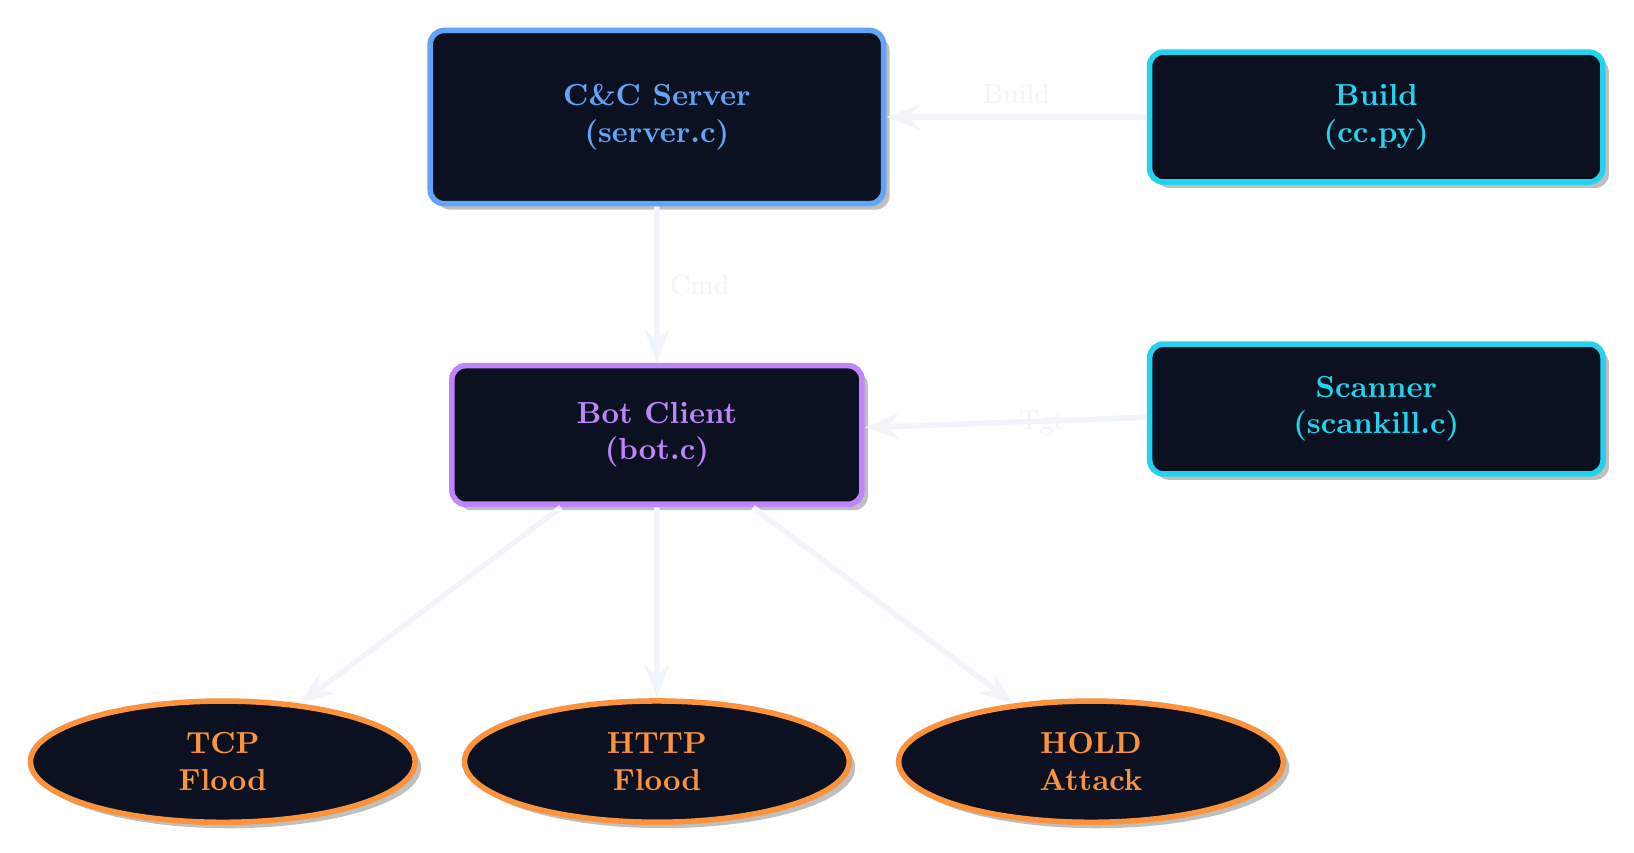
\begin{tikzpicture}[
            scale=1.1, transform shape,
            node distance=2cm and 2.5cm,
            >=Stealth,
            server/.style = {rectangle, draw=AccentBlue, fill=DarkBackground, text width=5cm, align=center, rounded corners=5pt, minimum height=2cm, font=\normalsize\bfseries, text=AccentBlue, line width=2pt, drop shadow},
            client/.style = {rectangle, draw=AccentPurple, fill=DarkBackground, text width=4.5cm, align=center, rounded corners=5pt, minimum height=1.6cm, font=\normalsize\bfseries, text=AccentPurple, line width=2pt, drop shadow},
            module/.style = {rectangle, draw=AccentCyan, fill=DarkBackground, text width=5cm, align=center, rounded corners=5pt, minimum height=1.5cm, font=\normalsize\bfseries, text=AccentCyan, line width=2pt, drop shadow},
            attack/.style = {ellipse, draw=AccentOrange, fill=DarkBackground, text width=3cm, align=center, minimum height=1.4cm, inner sep=2pt, font=\normalsize\bfseries, text=AccentOrange, line width=2pt, drop shadow},
            connection/.style = {draw, ->, line width=2pt, TextWhite}
        ]
            \node [server] (cnc) {C\&C Server\\ (server.c)};
            \node [client, below=1.8cm of cnc] (bot) {Bot Client\\ (bot.c)};
            \node [module, right=3cm of cnc] (build) {Build\\ (cc.py)};
            \node [module, below=1.8cm of build] (scanner) {Scanner\\ (scankill.c)};
            \node [attack, below=2.2cm of bot] (http) {HTTP\\ Flood};
            \node [attack, left=0.5cm of http] (tcp) {TCP\\ Flood};
            \node [attack, right=0.5cm of http] (hold) {HOLD\\ Attack};
            
            \draw [connection] (cnc) -- node[right, font=\small, text=TextWhite] {Cmd} (bot);
            \draw [connection] (build) -- node[above, font=\small, text=TextWhite] {Build} (cnc);
            \draw [connection] (scanner) -- node[right, font=\small, text=TextWhite] {Tgt} (bot);
            \draw [connection] (bot) -- (tcp);
            \draw [connection] (bot) -- (http);
            \draw [connection] (bot) -- (hold);
        \end{tikzpicture}
        
        \vspace{0.8em}
        \begin{minipage}{0.95\linewidth}
            \normalsize
            The architecture follows a centralized C2 model [1]. The \texttt{server.c} component manages the botnet via TCP port 1994, while \texttt{bot.c} resides on infected devices. The \texttt{cc.py} build system is crucial for cross-compiling payloads for various architectures.
        \end{minipage}
    }

    % ==========================================================================
    % COLUMNA 2
    % ==========================================================================
    \column{0.33}

    \block{Infection Process Flow}{
        \centering
        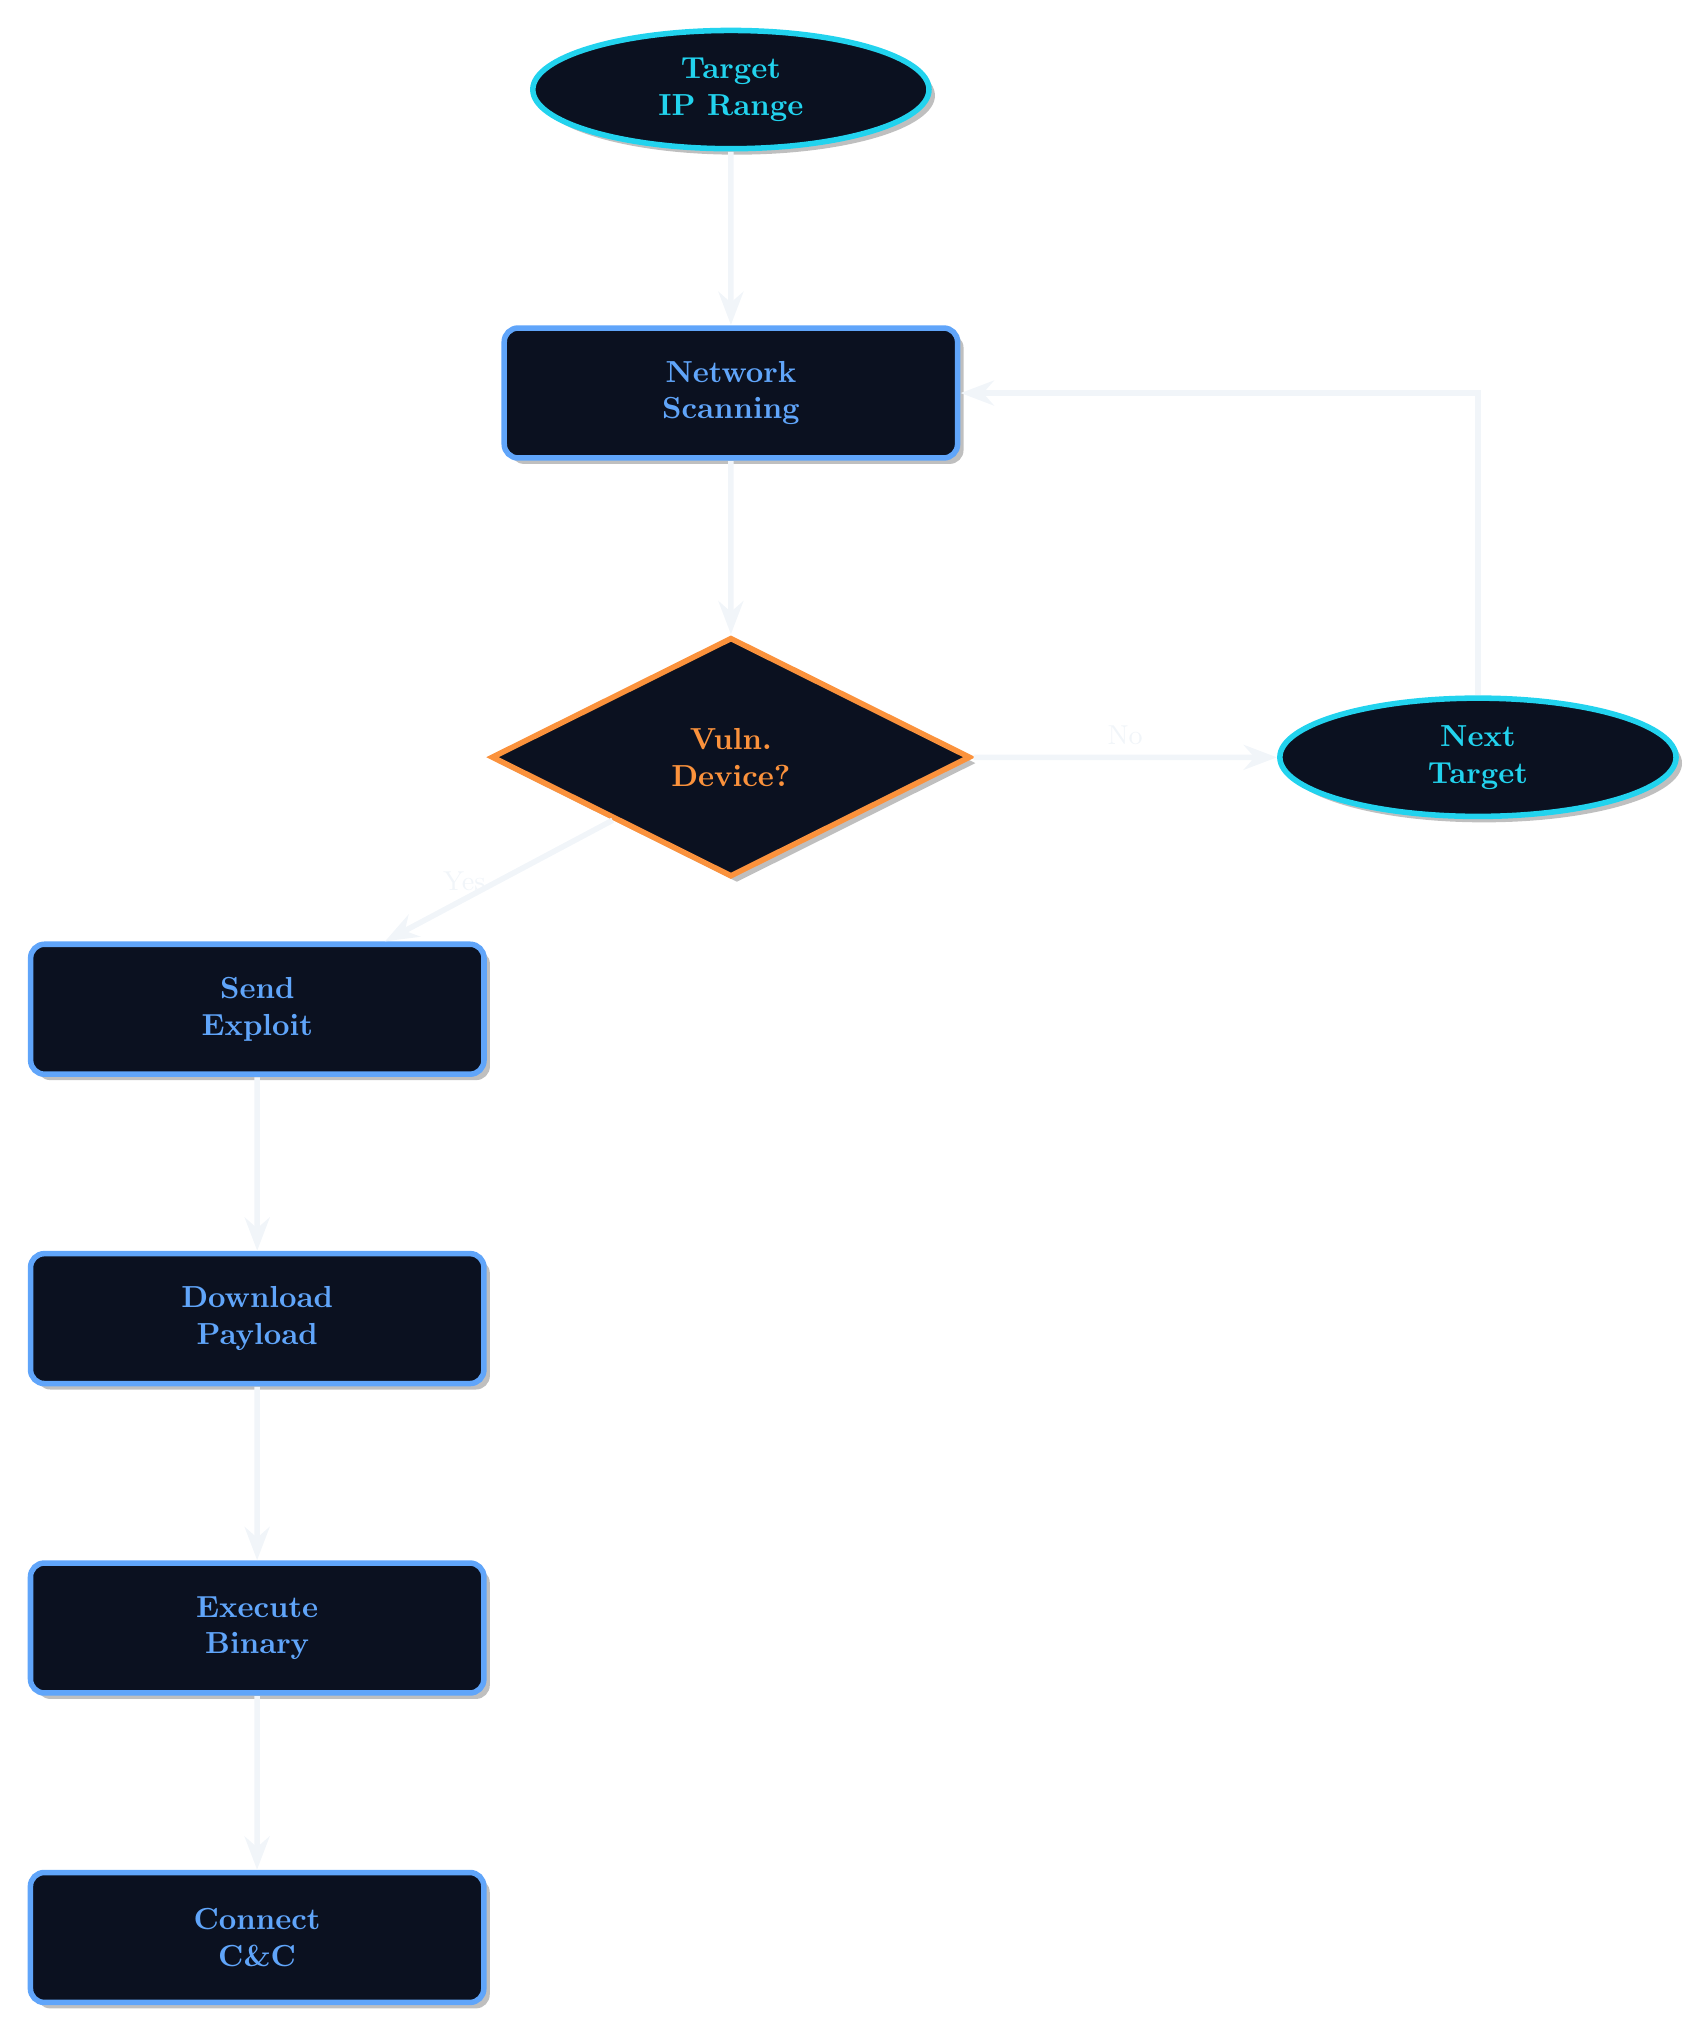
\begin{tikzpicture}[
            scale=1.1, transform shape,
            node distance=2cm, auto, >=Stealth,
            process/.style = {rectangle, draw=AccentBlue, fill=DarkBackground, text width=5cm, text centered, rounded corners=5pt, font=\normalsize\bfseries, text=AccentBlue, minimum height=1.5cm, line width=2pt, drop shadow},
            decision/.style = {diamond, draw=AccentOrange, fill=DarkBackground, text width=3.5cm, text centered, aspect=2, font=\normalsize\bfseries, text=AccentOrange, line width=2pt, drop shadow},
            data/.style = {ellipse, draw=AccentCyan, fill=DarkBackground, text width=3cm, text centered, font=\normalsize\bfseries, text=AccentCyan, line width=2pt, drop shadow},
            arrow/.style = {draw, ->, line width=2pt, TextWhite}
        ]
            \node [data] (start) {Target\\IP Range};
            \node [process, below=of start] (scan) {Network\\Scanning};
            \node [decision, below=of scan] (vuln) {Vuln.\\Device?};
            \node [process, below left=of vuln] (exploit) {Send\\Exploit};
            \node [process, below=of exploit] (payload) {Download\\Payload};
            \node [process, below=of payload] (execute) {Execute\\Binary};
            \node [process, below=of execute] (connect) {Connect\\C\&C};
            \node [data, right=3.5cm of vuln] (next) {Next\\Target};
            
            \draw [arrow] (start) -- (scan);
            \draw [arrow] (scan) -- (vuln);
            \draw [arrow] (vuln) -- node[left, font=\small, text=TextWhite] {Yes} (exploit);
            \draw [arrow] (vuln) -- node[above, font=\small, text=TextWhite] {No} (next);
            \draw [arrow] (next) |- (scan);
            \draw [arrow] (exploit) -- (payload);
            \draw [arrow] (payload) -- (execute);
            \draw [arrow] (execute) -- (connect);
        \end{tikzpicture}
        
        \vspace{0.8em}
        \begin{minipage}{0.95\linewidth}
            \normalsize
            The infection cycle begins with network scanning (\texttt{scankill.c}) to identify vulnerable devices. Upon successful exploitation (e.g., via Telnet brute-force or specific CVEs), the payload is downloaded and executed, establishing a persistent connection to the C2 server [2].
        \end{minipage}
    }



    \block{Security Risk Assessment}{
        \centering
        \normalsize
        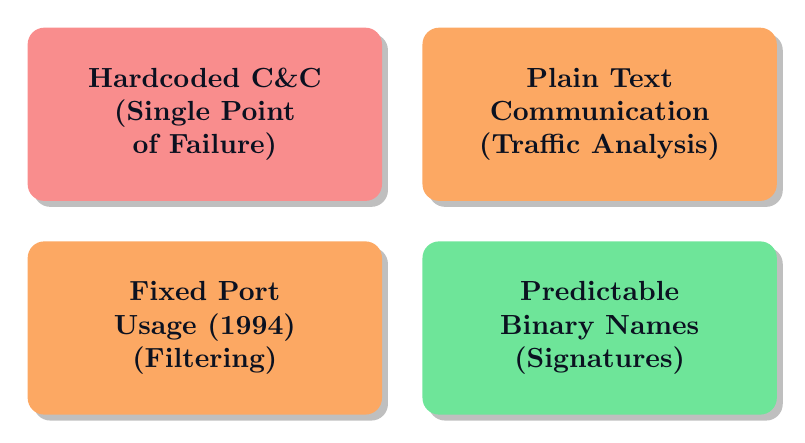
\begin{tikzpicture}[
            box/.style={rectangle, draw=none, minimum width=4.5cm, minimum height=2.2cm, align=center, font=\normalsize\bfseries, rounded corners=6pt, drop shadow},
            high/.style={fill=AccentRed!80, text=DarkBackground},
            med/.style={fill=AccentOrange!80, text=DarkBackground},
            low/.style={fill=AccentGreen!80, text=DarkBackground}
        ]
            \node[box, high] (topleft) at (0,0) {Hardcoded C\&C\\(Single Point\\of Failure)};
            \node[box, med, right=0.5cm of topleft] (topright) {Plain Text\\Communication\\(Traffic Analysis)};
            \node[box, med, below=0.5cm of topleft] (bottomleft) {Fixed Port\\Usage (1994)\\ (Filtering)};
            \node[box, low, right=0.5cm of bottomleft] (bottomright) {Predictable\\Binary Names\\(Signatures)};
        \end{tikzpicture}
        
        \vspace{0.5em}
        \begin{minipage}{0.95\linewidth}
            \normalsize
            \textbf{High Risk:} Hardcoded IP addresses allow defenders to sinkhole the entire botnet.
            \textbf{Medium Risk:} Lack of encryption enables traffic inspection and signature generation.
        \end{minipage}
        \vspace{2.5cm} % Padding for alignment
    }

    \block{Multi-Architecture Support}{
        \centering
        \normalsize
        \renewcommand{\arraystretch}{1.8}
        \begin{tabular}{p{0.45\linewidth}p{0.45\linewidth}}
            \rowcolor{DarkBackground}
            \textbf{\color{AccentCyan}MIPS:} Routers, Network Equip. & \textbf{\color{AccentPurple}ARM:} IoT Devices, IP Cameras \\
            \rowcolor{DarkBackground}
            \textbf{\color{AccentCyan}x86/x64:} PC-based IoT Systems & \textbf{\color{AccentPurple}PowerPC:} Legacy Embedded \\
            \rowcolor{DarkBackground}
            \textbf{\color{AccentCyan}SPARC:} Enterprise IoT Devices & \textbf{\color{AccentPurple}SH4:} Multimedia Devices \\
        \end{tabular}

        \vspace{1em}
        \colorbox{BlockBackground}{\parbox{0.9\linewidth}{\centering\large
        \textbf{\color{AccentCyan}12 architectures supported} - Massive IoT attack surface
        }}
        
        \vspace{1em}
        \begin{minipage}{0.95\linewidth}
            \normalsize
            Unlike early IoT botnets that targeted specific platforms, SlumX supports 12 distinct architectures including MIPS, ARM, and x86 [3]. This broad compatibility significantly increases the potential infection pool, as noted in recent IoT statistics [5].
        \end{minipage}
    }

    % ==========================================================================
    % COLUMNA 3
    % ==========================================================================
    \column{0.33}

    \block{Attack Vector Complexity}{
        \centering
        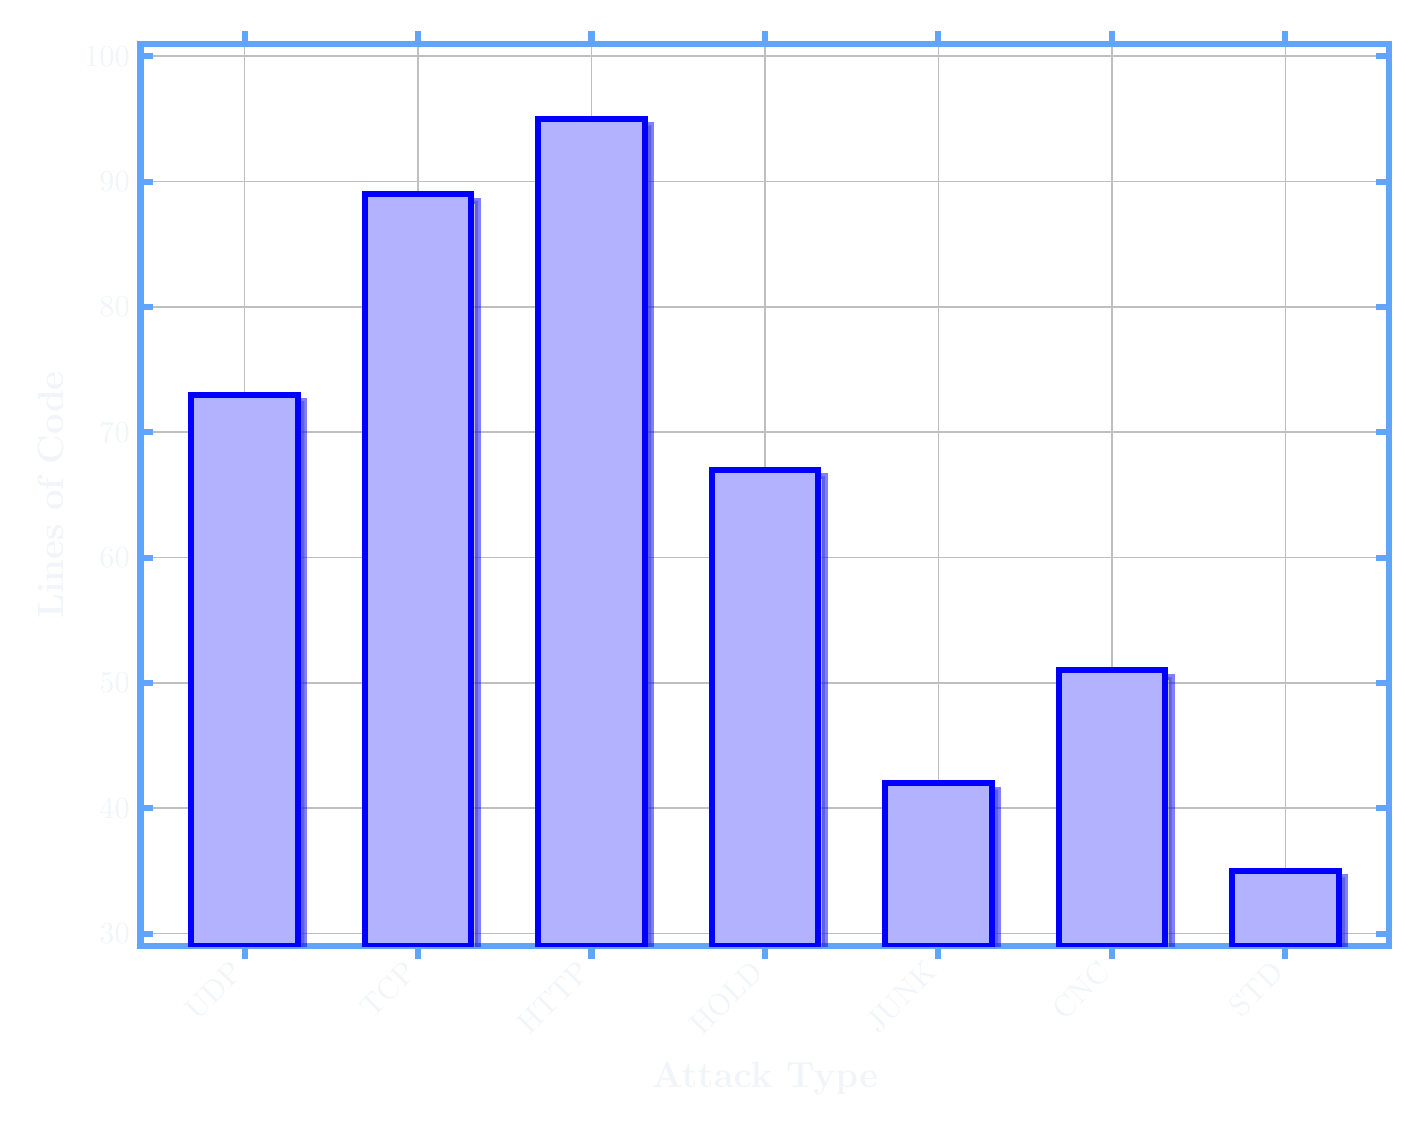
\begin{tikzpicture}[scale=1.1, transform shape]
        \begin{axis}[
            xlabel={\textbf{\color{TextWhite}Attack Type}},
            ylabel={\textbf{\color{TextWhite}Lines of Code}},
            symbolic x coords={UDP,TCP,HTTP,HOLD,JUNK,CNC,STD},
            xtick=data,
            ybar,
            bar width=35pt,
            grid=major,
            grid style={line width=0.5pt, draw=gray!50},
            width=16cm,
            height=12cm,
            x tick label style={rotate=45, anchor=east, font=\normalsize, color=TextWhite},
            y tick label style={font=\normalsize, color=TextWhite},
            axis line style={line width=2pt, draw=AccentBlue},
            tick style={line width=2pt, draw=AccentBlue},
            label style={font=\large, text=TextWhite},
            every axis plot/.append style={fill=AccentPurple!80, draw=AccentPurple, line width=2pt, drop shadow}
        ]
        \addplot coordinates {(UDP,73) (TCP,89) (HTTP,95) (HOLD,67) (JUNK,42) (CNC,51) (STD,35)};
        \end{axis}
        \end{tikzpicture}
        
        \vspace{0.5em}
        {\normalsize\color{TextWhite} HTTP-based attacks show highest complexity (95 LOC).}
        
        \vspace{1em}
        \begin{minipage}{0.95\linewidth}
            \normalsize
            The botnet supports multiple DDoS vectors. Analysis shows that HTTP floods are the most complex to implement (95 LOC), requiring valid header construction to bypass simple filters. In contrast, UDP and TCP floods rely on raw socket manipulation for high-volume traffic generation [3].
        \end{minipage}
    }

    \block{Key Findings \& Conclusions}{
        \normalsize
        \begin{itemize}\setlength\itemsep{0.6em}
            \item \textbf{\color{AccentCyan}Multi-architecture:} 12 architectures (MIPS, ARM, x86, embedded) dramatically expanding attack surface.
            \item \textbf{\color{AccentPurple}Advanced evasion:} Process masquerading, anti-analysis features, IoT-specific hiding techniques.
            \item \textbf{\color{AccentOrange}Targeted exploitation:} Vendor-specific exploits showing evolution to targeted attacks.
            \item \textbf{\color{AccentRed}Future Trends:} Mirai-driven botnets are moving toward more sophisticated infrastructures with increased persistence [4].
        \end{itemize}

        \vspace{1em}
        \colorbox{BlockBackground}{\parbox{0.96\linewidth}{\normalsize\color{AccentCyan}
        \textbf{Future Research:}
        \vspace{0.2em}
        \begin{itemize}\setlength\itemsep{0.3em}
            \item Dynamic analysis frameworks
            \item Specialized detection technologies [4]
        \end{itemize}
        }}
    }

    \block{References}{
        \normalsize
        \begin{itemize}\setlength\itemsep{0.4em}
            \item[1] M. Antonakakis et al., "Understanding the Mirai Botnet," \emph{USENIX Security}, 2017.
            \item[2] A. Marzano et al., "The evolution of bashlite and mirai IoT botnets," \emph{IEEE S\&P}, 2018.
            \item[3] G. Vishwakarma and G. S. Chhabra, "Targeted DDoS Attacks on IoT: A Survey of the Mirai Botnet and its Variants," \emph{AISC}, 2023.
            \item[4] A. D. Alghazzawi et al., "An Efficient Hybrid Deep Learning Model for Detecting IoT Botnet Attacks," \emph{IEEE Access}, 2024.
            \item[5] Statista, "IoT connected devices installed base worldwide," 2024.
        \end{itemize}
        
        \vspace{1em}
        \begin{center}
        \textbf{\large\color{AccentBlue}Research Paper Access}\\
        \vspace{0.5em}
        
\includegraphics[width=5cm]{QR_research.png}
        \end{center}
        \vspace{0.5cm} % Minor padding
    }

\end{columns}

\end{document}
